% !TEX encoding = UTF-8 Unicode
% !TEX TS-program = pdflatex
% !TEX spellcheck = en_US


% In order to correctly compile this document,
% execute the following commands:
% 1. pdflatex
% 2. pdflatex
% 3. pdflatex



\documentclass[amsthm,ebook]{saparticle}

% IF YOU USE PDFLATEX
\usepackage[utf8x]{inputenc}
% if you write in english and in greek
\usepackage{ucs}
\usepackage[greek,english]{babel}
\languageattribute{greek}{polutoniko}

% IF YOU USE XELATEX
%\usepackage{polyglossia}
% if you write in italian
%\setmainlanguage{english}
% If you want put some ancient greek:
%\setotherlanguage[variant=polytonic]{greek}
%\newfontfamily{\greekfont}[Ligatures=TeX]{Palatino Linotype}

% dummy text (remove in a normal thesis)
% remove if not necessary
\usepackage{siunitx}
%Natbib for bibliography management
\usepackage[authoryear]{natbib}
% custom commands
\newcommand{\bs}{\textbackslash}

\usepackage{fontspec}

\usepackage{polyglossia}

\setmainlanguage{english}
\setotherlanguage{greek}

\newfontfamily\greekfont[Script=Greek]{CMU Serif}

%\setmainfont{lmr}
%%%%%%%%
%TITLE:%
%%%%%%%%
\title{Towards a Universal Facebook of the Ancient World}
\author[KU]{Yanne Broux\corref{first}}
\address[KU]{KU Leuven / Research Foundation Flanders (FWO)}
\cortext[first]{Corresponding author. Email: Email: yanne.broux@kuleuven.be}
\date{2015-09-16}
\begin{document}

\maketitle

\begin{abstract}
Facebooking the past. The idea grew while developing a database of all people mentioned in texts from Greco-Roman Egypt
(350 BC–AD 800). Thanks to Trismegistos' role in EAGLE, Named Entity Recognition can now be applied to almost 500,000
Latin inscriptions from the Roman Empire, and some 400,000 clusters containing personal names can be extracted. This
collection of names will lead to a large-scale study of naming practices in the ancient world, and how these reflect
changes in society at large.
\end{abstract}
\keywords{Latin epigraphy, Trismegistos, Named Entity Recognition, Social Network Analysis, Onomastics, Prosopography}




\section{Trismegistos: the early years}


\noindent Facebooking the past. The idea grew a couple of years ago, while developing a database of all people mentioned in texts
from Greco-Roman Egypt. While probably not exactly considered Big Data by those who actually work with BIG data, the
500,000 or so attestations of individuals in Trismegistos open up some prospects for quantitative analysis, something
historians still tend to shy away from. One of the approaches I have been exploring is Social Network Analysis [SNA].
SNA was developed in the 1960s in mathematics, anthropology and sociology and measures structural forms of relations
between individuals, places and/or events. Over the past couple of decades, it has found its way to numerous other
fields, such as physics, neuroscience, and recently also (modern) history. Within ancient history, however, SNA still
needs to obtain a firm footing.

To reconstruct proper social networks, a decent prosopography is indispensable. In a traditional scholarly setting, this
implies time-consuming and painstaking manual labor. Fortunately, in a digital environment, there are other ways, and
Trismegistos (\url{www.trismegistos.org}) forms an ideal starting point. Trismegistos grew out of a long tradition of
databases and prosopographies (structured lists of people), as well as various other Ancient History projects at KU
Leuven. The original idea of Trismegistos was to foster interdisciplinarity in the study of Ancient Egyptian society by
creating a central database with metadata about published papyrological texts from Greco-Roman Egypt, in a first
instance written in Greek, Latin and Egyptian (including hieroglyphic, hieratic and demotic). The inclusion of Egyptian
soon dissolved the disciplinary boundary with epigraphy, broadened the chronological window, which was eventually set
to 800 BC – AD 800, and led to the inclusion of further languages such as Coptic, Aramaic and Arabic.

Apart from texts, since 2008 Trismegistos also intensively deals with places and people. Building on open access to the
full text in repositories, Named Entity Recognition procedures are used to create lists of toponyms and anthroponyms
that occur in the ancient sources. This was first applied during the socio-onomastic project `Creating Identities in
Graeco-Roman Egypt' (KU Leuven OT project 2008-2012), on a corpus of about 50,000 papyri and ostraca in the Duke
Databank of Documentary Papyri (\url{papyri.info}). With the additional support of a Hercules Grant, (`An Interdisciplinary
Database of Proper Names in Late Pharaonic, Graeco-Roman and Byzantine Egypt (ca. 800 BC – AD 640)'; 2008-2014) the
work on the core data could be finished in just over two years, resulting in a database with almost half a million
references to people (Trismegistos People) and an additional hundred-thousand or so place names (Trismegistos Places)
mentioned in texts from Egypt.

On the basis of Trismegistos People, several studies on naming practices, modes of identification and identity issues in
Greco-Roman Egypt have been published. Two PhDs focused on the longstanding tradition of double names: the first dealt
with the Ptolemaic period, when this form of polyonymy served to cross ethnic borders \citep{Coussement}, the
other with the Roman period, when the practice was adapted by the local elite to distinguish themselves from the \emph{hoi
polloi} and to resemble Roman nomenclature \citep{Broux2015a}. The data of the fourth century AD provided new insights into
the spread of Christianity in Egypt \citep{Depauw2013}. The development of a standardized identification
cluster, consisting of a person's name, patronymic and metronymic \citep{BrouxDepauw}, as well as the use of fixed
expressions to denote illegitimacy \citep{Broux2015b}, name change \citep{Broux2013a} and official identification \citep{Broux2010}, were all related to the legal reorganization of the population under the Romans and the
ensuing tax reform \citep{Broux2013b}. Most recent studies focus on the influence of Roman socio-linguistic practices on
Greek and Egyptian conventions \citep{Depauw} and how network analysis can provide us with new insights regarding
onomastic habits and what they say about cultural identity and social status \citep{Broux2015c}.

\section{Going global: an encompassing source guide for the ancient world}


\subsection{Expanding Trismegistos Texts}


\noindent Like Facebook, however, Trismegistos wants to grow, and get the entire ancient world on board. To achieve this goal,
Trismegistos' core database, the text database, must first be expanded by broadening its chronological and geographic
horizon. Since 2013 the team has been actively working toward the inclusion of all texts from antiquity in
Trismegistos. This implies including Latin and Greek inscriptions, an estimated 700,000 texts. Contacts with the Latin
epigraphic database in Heidelberg resulted in Trismegistos' participation in the Europeana EAGLE project, coordinating
the disambiguation across all partners. This added about 150,000 new texts to the Trismegistos database. The remaining
300,000 will be integrated from another source (Clauss-Slaby: \url{www.manfredclauss.de}), so that the coverage of Latin will
soon be exhaustive. For Greek, good contacts have been established with the main players in the field (PHI:
\url{epigraphy.packhum.org/inscriptions/}; DC3 [i.e. Duke, SEG, Claros]: \url{blogs.library.duke.edu/dcthree/}), and the aim is to
become partners in a project dealing with the 250,000 or so inscriptions during the next year. At the same time
Trismegistos is also working towards a complete coverage of indigenous languages and scripts, which are often separate
fields, isolated from the `classical' world. New partnerships for Etruscan have been set up, and soon also for Punic
(CIP: \url{cip.cchs.csic.es}) and South-Arabian (DASI: \url{dasi.humnet.unipi.it}), while for the Italic languages, for Gallic,
Lepontic, Venetic, and Messapian information has already been digitized on the basis of existing corpora.




\subsection{Expanding Trismegistos People}


\noindent With the experience obtained during the extraction of names from the Greek papyri, Named Entity Recognition will be
applied to the Latin inscriptions incorporated in Trismegistos so far. This will result in the addition of an estimated
500,000 or more new references to names/individuals to Trismegistos People. Network analysis will be used to help with
the disambiguation of individuals.




\subsubsection{Named Entity Recognition}


\noindent The collection of references to people and their names in the inscriptions will be carried out by applying Named Entity
Recognition [NER] to the clusters of capitalized words extracted from the full text repositories of Greek and Latin
inscriptions.

NER was originally developed by computational linguists in the 1990s to detect and classify pre-defined elements in
texts, but quickly spread to other fields, such as biology and genetics, and is now gaining momentum in the Digital
Humanities \citep{vanHooland}. The problem with NER-systems, however, is that techniques designed for one
genre or field do not necessarily work for others, due to specific text properties (some follow strict writing
constraints, e.g. scientific or news articles, while others, such as email or tweets, are more informal), or due to
language-related grammatical and syntactical formats.

For ancient Greek and Latin, the languages of the inscriptions under scrutiny here, there were no ready-to-use NER
solutions. In a case language, proper names are more variable; the different accents on vowels make letters less easily
recognizable; and in particular the onomastic system and the way people are identified is completely different from
modern languages. Therefore a strategy needed to be developed to cope with the multilingualism of the sources and the
declensions of the inflected languages. 

Trismegistos opted for a combination of a gazetteer and a rule-based approach. For the gazetteer a three-tiered
onomastic database structure was developed in Trismegistos People, dealing with names, name variants, and declined name
variants respectively. The first database, NAM, currently has 34,106 entries, e.g. the name Isidoros. Each name is
connected to a set of variants in all possible languages. As a rule, only very minor dialectal or orthographical
variation is allowed in the `native' language, in this case Greek (e.g. \textgreek{Εἰσίδωρος} and \textgreek{Ἰσίδορος}). Many of the variants are actually created by renderings of a name in other languages, e.g. %{\fontspec{Liberation Sans}ȝysydwrs}
Ỉsytrs, {\fontspec{Gentium}ȝysydwrs} or {\fontspec{ArialCoptic} ⲓⲥⲓⲇⲱⲣⲉ} in Egyptian and Coptic. In all there
are 177,290 variants in the NAMVAR database. Finally, for each of the variants, the declined forms were created, e.g.
\textgreek{Ἰσίδωρου}) or \textgreek{Ἰσίδωρωι} (dative). This NAMVARCASE database is the largest with
667,677 entries, and this set is used as a gazetteer for NER. It was developed on the basis of the set of names of some
40,000 individuals with titles listed in the Prosopographia Ptolemaica (KU Leuven) and was supplemented with new names
collected during the `Creating Identities' project \citep{Depauw2009}. Through cooperation with the Lexicon of
Greek Personal Names (Oxford University) the names of some 300,000 individuals can now also be integrated.

Apart from this gazetteer, rules were developed to cope with the combination of names, or more correctly declined name
variants, as well as with the combination of names with non-onomastic introductory terms (e.g. `son of') in the
identification of individuals. For Greek texts, this is pretty straightforward, as people were identified by their name
(generally a single name, in some cases a double name) followed by genealogical identifiers (in the genitive form)
only. The onomastic habits encountered in Latin inscriptions differ significantly, however. Here the majority of the
individuals follow the Roman naming system. This consists of a fossilized praenomen, a nomen gentilicium (the
equivalent of our family name), and a personal cognomen. Often the patronymic was inserted between the gentilicium and
cognomen; sometimes even the papponymic and the voting tribe, e.g. \emph{Marcus Tullius Marci filius Marci nepos Cornelia
Cicero} (`Marcus Tullius Cicero, son of Marcus, grandson of Marcus, [of the] Cornelia [tribe]'). A completely new set of
rules is therefore being developed to apply to the Latin inscriptions.




\subsubsection{Human quality control and prosopographical identifications}


\noindent Once the clusters of capitalized words have been extracted and have been matched to the onomastic gazetteer and rules
for name combinations, a human check will be performed. This includes tasks which are not easily automated:
interpreting declined name variants as attestations of a specific case where the mere form is ambiguous; deciding
whether some ambiguous entries are toponyms or anthroponyms; and reviewing the results of the cluster interpretation
rules and adding relevant information where necessary. 

All this could be labeled `quality control', but we will also rely exclusively on humans for the logical next step when
developing a prosopography: the identification of namesakes as attestations of the same person. Since the systematic
review will be performed text per text, only intratextual identifications can be implemented at this stage.




\subsubsection{Social Network Analysis}


\noindent Social Network Analysis [SNA] was developed in the 1960s in mathematics, anthropology and sociology and measures
structural forms of relations between individuals. It has huge potential for future historical research, not only by
applying `traditional' network analysis for the study of social interaction, but also by developing new,
non-conventional techniques.

In the wake of the automatic extraction of individuals from Greek papyri during the `Creating Identities' project,
people appearing in more than one text could not be identified and were therefore entered in Trismegistos People under
multiple records. The identification of these doubles is a difficult and time-consuming process, not in the least
because of the high degree of homonymy: in village communities, similar names were common, and in families, names were
often passed down every other generation. This makes it difficult to distinguish between one person and another. Broux
and Vanbeselaere therefore developed a new procedure to identify individuals with the help of graph visualization and
SNA \citep{BrouxVanbeselaere}. By linking people based on co-occurrence in the same texts, an overview of
all the data is presented in a single network, where one can ``zoom in'' on specific individuals and compare their
``surroundings''. When specific clusters of names reappear, these are likely the same individuals mentioned in different
texts (see Fig.~\ref{fig:1}: each circle [or `node'] represents an individual; some of these need to be merged, since they
actually refer to the same person). 




\begin{figure}[!bp]
\centering
 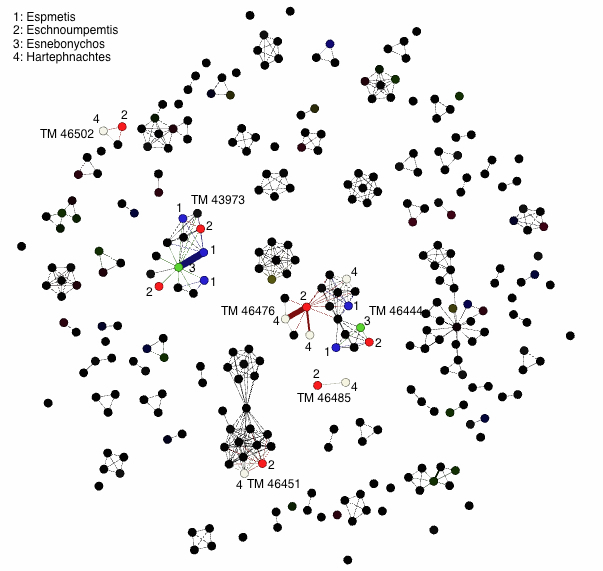
\includegraphics[width=\columnwidth]{EAGLE2016FullPaperBroux-img001.jpg}
\caption{Visualizing individuals co-occurring in texts. }
\label{fig:1}
\end{figure}







Additionally, the developed identification method enables us to discern family components. Mapping genealogical
relationships is often problematical, especially when individuals are attested in different capacities. Someone who is
mentioned as the father of an athlete in a victory list is not easily recognized as the state official in a petition.
In other words, social and professional links do not always overlap with family ties, and these need to be synced to
provide a complete picture and to prepare the data for the next step: analyzing networks of names.

The application of SNA to onomastics is another avenue that has not yet been explored. By linking names on the basis of
genealogical relations (since names are the result of conscious choices made by parents), the co-occurrence of names in
communities can be mapped, which opens up new possibilities for quantification and interpretation \citep{Broux2015c}. A
name's popularity can be calculated by means of its in-degree (i.e. how many other names point to it), while the
density of the network, the number of reciprocal links and the weight of these links can tell us something about the
social motives behind these naming patterns. For the local elite of Roman Egypt, for example, descent was of prime
importance, since membership was strictly hereditary, and by limiting themselves to a specific collection of names,
they could express family and community ties. Moreover, networks like these can help us evaluate the perception of
names in antiquity, as well as determine the linguistic origins of undefined names, on the basis of their location in
the graph.

\section{Goals}
\subsection{Study of naming practices}


\noindent The collection of names from across the entire Mediterranean will lead to a large-scale study of naming practices in the
ancient world, and how these reflect changes in society at large. A major transition point is of course the steady
integration of regions and states across the Mediterranean and Western Europe into the Roman Empire. The focal point
will therefore be the impact of the Roman occupation on traditional naming and identification conventions in different
provinces. Regions where pre-Roman material is also available (e.g. Gaul, Magna Graecia, Asia Minor) are especially
significant when mapping aspects of continuity and change chronologically. Moreover, results from both eastern and
western provinces will be compared to study uniformization, whether imposed from above or spread out from below.




\subsection{Towards a Facebook of the ancient world}


\noindent Eventually, the goal of Trismegistos is to recreate a prosopography of the Greco-Roman world. Reconstructing social
networks of the past will help us gain a better understanding of the mechanisms of interaction in the ancient
Mediterranean, not only on the micro level (individuals), but also on the mesa (communities) and even macro (regions,
empires) levels. At the same time connections and communication across these different levels can be analyzed: how
individuals, as members of local communities, were integrated into larger political structures (top-down approach), and
how these communities responded to impositions from above (bottom-up approach). Social models, such as the six degrees
of separation theory, can be tested, to check whether our `small world' perception is indeed the result of present-day
technology and mass-communication, or if similar structures of interconnectivity existed, and, if so, what the
conditions for this ancient globalization were back then. Mark Zuckerberg out. Enter Trismegistos. 


\bibliographystyle{sapauth-eng}
\bibliography{../../EAGLE}

\end{document}
